%\section{Supplementary material 1 : Tree building}

\subsection{Morphological character states}
To obtain a realistic value for the probability of having \textit{k} characters states for each simulated morphological character, we randomly selected 100 morphological matrices, each with more than 100 characters each, from TreeBASE (\url{http://treebase.org/}). We only selected matrices published between 1985 and 2013 and covering 19 taxonomic classes (Chordata, Arthropoda, Annelida, Angiosperm, Gymnosperm and Pteridophyta). This resulted in a total of 22563 characters that had between two and 10 character states. We then extracted the proportion of characters with each number of states (two to 10) to give us an empirical estimate of the average number of character states for each character, as shown in Figure \ref{Fig_AppendixCharacters}. Most characters have two or three states, therefore we only simulate characters with two or three states, and sample these in proportion to their occurrence in our empirical data (probability of 0.85 for two states characters and 0.15 for three state characters). The code used for this section is available at \url{https://github.com/TGuillerme/Total_Evidence_Method-Missing_data/blob/master/Analysis/MorphologicalCharacterStates.R}.

\begin{figure}
\centering
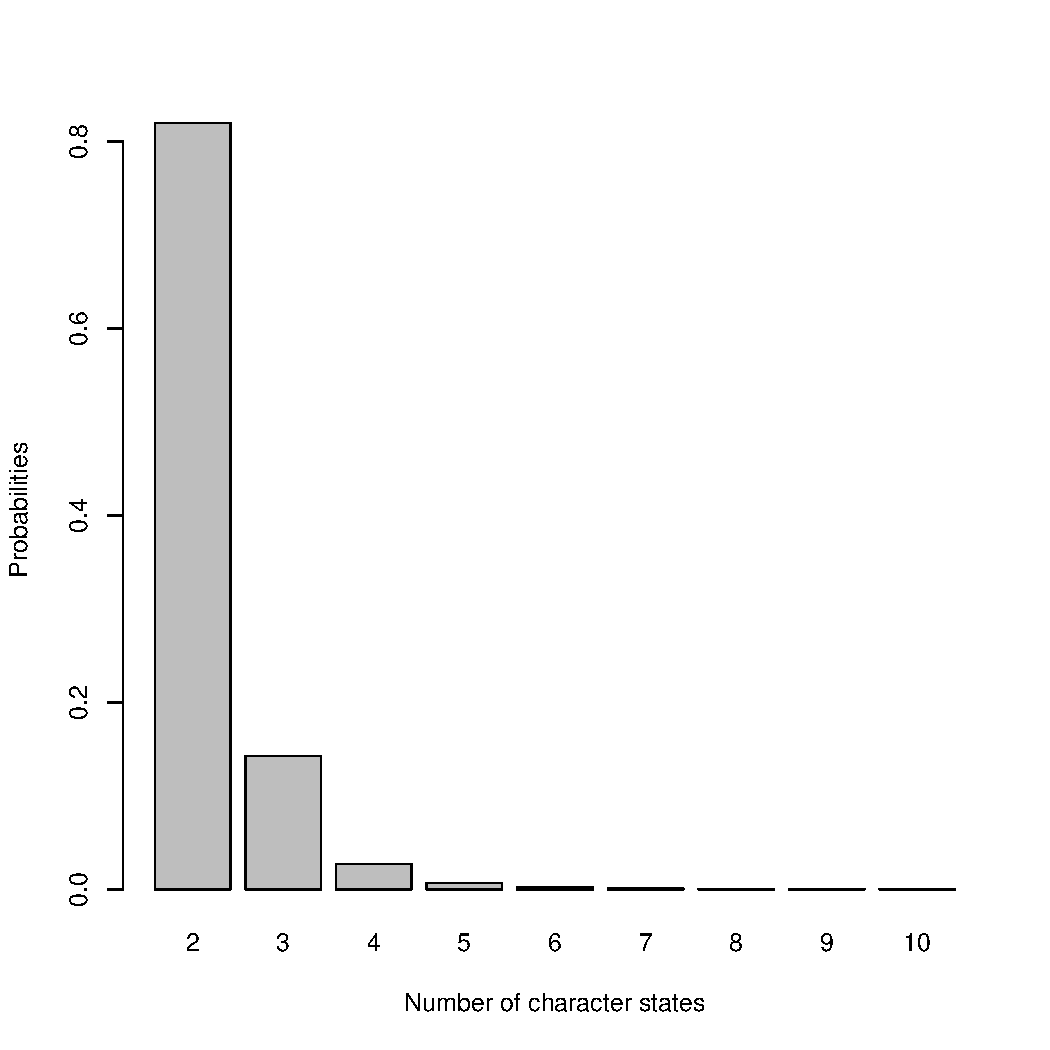
\includegraphics[keepaspectratio=true]{OnlineAppendices-LaTeXSuppFiles/SupplementaryFigures/TEM_Fig-AppendixCharacters.pdf}
\caption{The proportion of morphological characters with between two and 10 character states extracted from 100 randomly selected empirical matrices downloaded from TreeBASE.}
\label{Fig_AppendixCharacters}
\end{figure}

\newpage
\subsection{Tree Building Software settings}

For clarity we have provided the exact settings used in our tree building below.

\subsubsection{Maximum Likelihood: RAxML version 8.0.20 \citep{Stamatakis21012014}}

\begin{itemize}
  \item Molecular data: GTR + $\Gamma_4$ (-m GTRGAMMA)
  \item Morphological data: Mk + $\Gamma_4$ (-K MK)
  \item Support: Rapid Boostrap algorithm (LSR), 1000 replicates
\end{itemize}

\subsubsection{Bayesian: MrBayes version 3.2.1 \citep{Ronquist2012mrbayes}}

\begin{itemize}
  \item Priors: Molecular data
  \begin{itemize}
    \item Rates distribution shape ($\alpha$) = 0.5
    \item Transition/Transversion ratio = 2 ($\beta$(80,40))
    \item Starting tree: "True" tree topology with each branch length = 1
  \end{itemize}
  \item Priors: Morphological data
  \begin{itemize}
    \item rates distribution shape ($\alpha$) = 0.5
  \end{itemize}
  \item Models
  \begin{itemize}
    \item Molecular data: HKY + $\Gamma_4$
    \item Morphological data: Mk + $\Gamma_4$
  \end{itemize}
  \item MCMC
  \begin{itemize}
    \item Two runs
    \item Four chains per run
    \item Generations $<$ 5$\times$$10^7$
    \item Sample frequency = 1.05$\times$$10^4$
    \item ASDS diagnosis frequency = 5$\times$$1^4$
    \item ASDS $<$ 0.01
    \item ESS $>>$ 200
    \item Burnin = 25\%
  \end{itemize}
\end{itemize}